\documentclass[aps,prb,superscriptaddress,nofootinbib]{revtex4}
\usepackage{amsfonts}
\usepackage{amsmath}
\usepackage{amssymb}
\usepackage{graphbox}
\usepackage{graphicx}
\usepackage{caption}
\usepackage{bm}
\usepackage{bbm}
\usepackage{cancel}
\usepackage{color}
\usepackage{mathrsfs}
\usepackage[colorlinks,bookmarks=true,citecolor=blue,linkcolor=red,urlcolor=blue]{hyperref}
\usepackage{simpler-wick}
\usepackage{appendix}
\usepackage{float}
\usepackage{array}
\usepackage{booktabs}
\usepackage[export]{adjustbox}
\setlength{\parindent}{10 pt}
\setlength{\parskip}{2 pt}
\setcounter{MaxMatrixCols}{30}
\bibliographystyle{apsrev}
\newcommand{\RNum}[1]{\uppercase\expandafter{\romannumeral #1\relax}}
\newcommand{\normord}[1]{{:\mathrel{#1}:}}
\def\tbs{\textbackslash}
\def \tr{\operatorname{tr}}
\def \Tr{\operatorname{Tr}}


\begin{document}
\title{Bosonization}
\author{Jie Ren}


\maketitle


\tableofcontents

\section{Particle-Hole Excitations}

The low energy excitations are particle-hole modes:
\begin{equation}
	\rho_{k}^\dagger = \sum_{q} c_{q+k}^\dagger c_{q}, \quad
	\rho_{k} = \sum_{q} c_{q}^\dagger c_{q+k} = \rho_{-k}^\dagger.
\end{equation}
To simplify the discussion, here we consider only a single branch of Fermion. 
The generalization to multiple branches is trivial since the dispersion is the same.
The commutation relation between $\rho_k$ and $\rho_{k'}^\dagger$ is:\footnote{We use the identity $[AB,C] = A[B,C] + [A,C]B$ and $[A,BC]=\{A,B\}C - B\{A,C\}$.}
\begin{equation}
\begin{aligned}
	\left[\rho_{k}, \rho_{k'}^\dagger \right]
	&= \sum_{q_1, q_2} \left[c_{q_1}^\dagger c_{q_1+k}, c_{q_2+k'}^\dagger c_{q_2}\right] \\
	&= \sum_{q_1, q_2} \left\{c_{q_1}^\dagger \left[c_{q_1+k}, c_{q_2+k'}^\dagger c_{q_2}\right] +\left[c_{q_1}^\dagger, c_{q_2+k'}^\dagger c_{q_2}\right] c_{q_1+k}\right\} \\
	&= \sum_{q_1, q_2} \left\{ \delta_{q_1+k,q_2+k'} c_{q_1}^\dagger c_{q_2} -
		\delta_{q_1,q_2} c_{q_2+k'}^\dagger c_{q_1+k} \right\} \\
	&= \sum_{q}\left[c^\dagger_{q+k'-k} c_{q}-c^\dagger_{q+k'} c_{q+k}\right].
\end{aligned}
\end{equation}
For $k \ne k'$, it is clear that $[\rho_{k},\rho_{k'}^\dagger]=0$.
However, when $k = k'$, we should be careful about the subtraction, since it evolve two infinities of which the subtraction is ill-defined.


\subsection{Normal Ordering}
Here we deal with the infinity with the lattice regularization, i.e., we think of the linearized theory as the low-energy approximation of a lattice mode, where the dispersion form a single energy band.
The left/right movers are actually in a single band but with positive/negative momentum.
Consider for example the density operator for the right mover, the commutator of the right moving density operator is then
\begin{equation}
	\left[\rho_{k,r}, \rho_{k,r}^\dagger \right] = \sum_{0<q<\pi} [n_{q,r}-n_{k+q,r}].
\end{equation}

\begin{figure}
	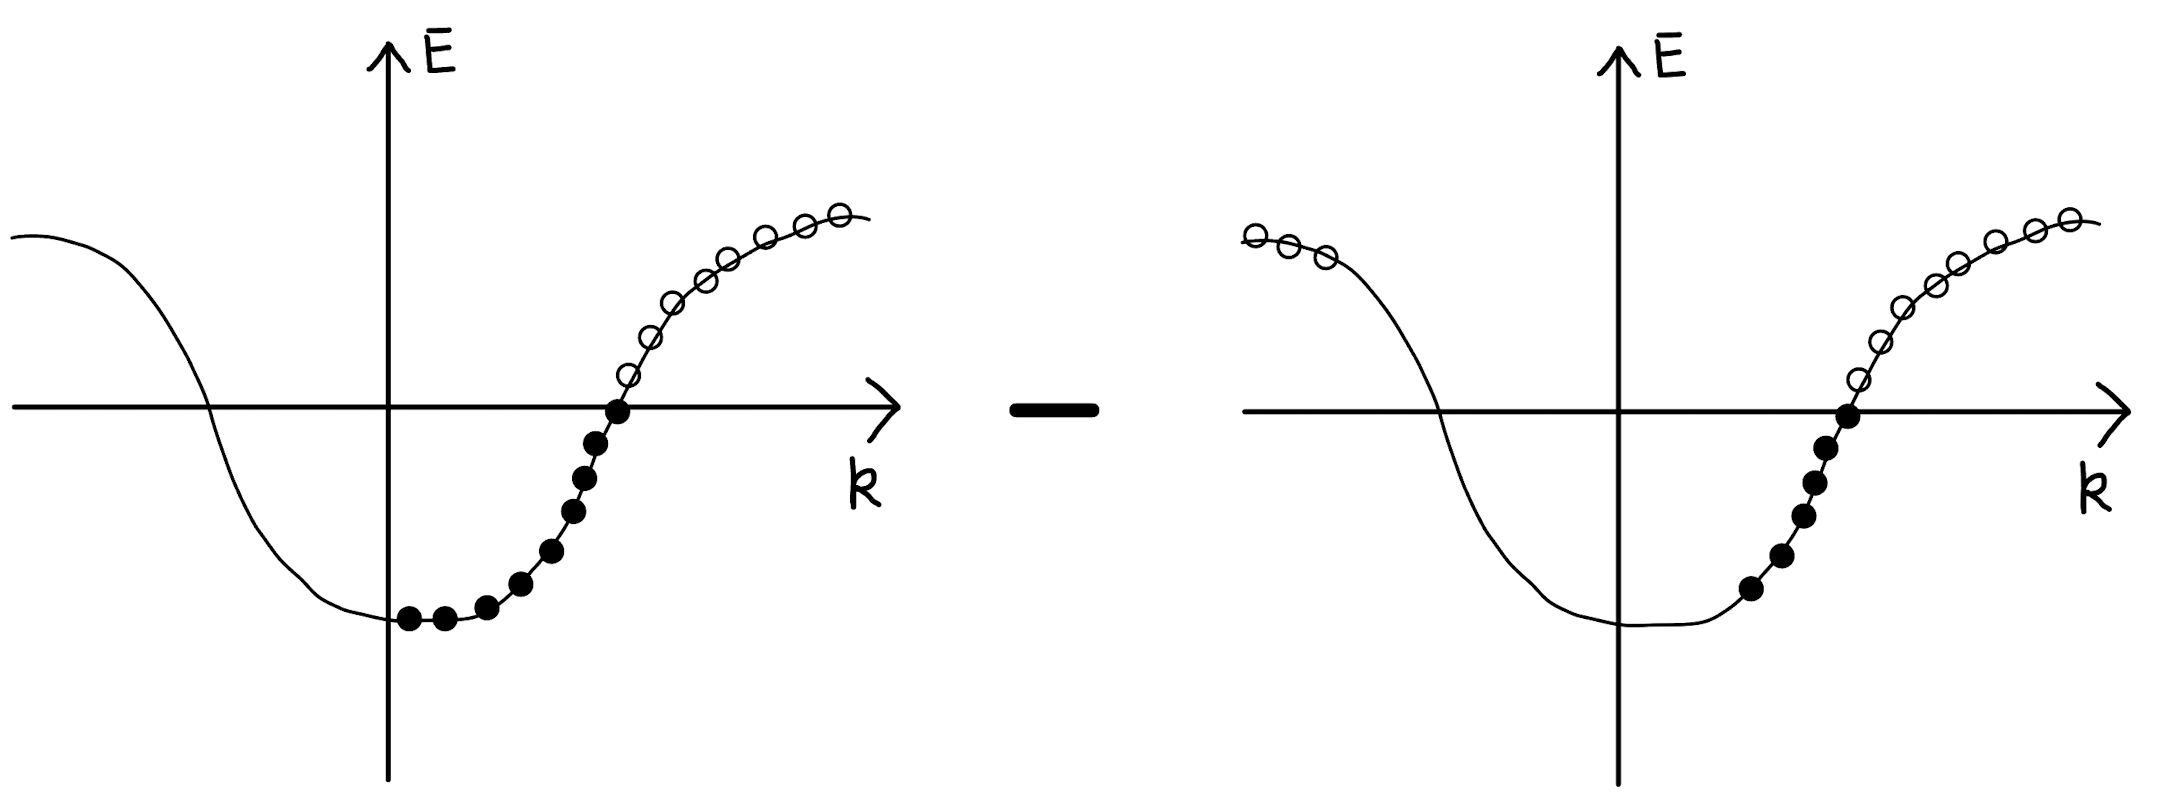
\includegraphics[hsmash=c,width=0.5\linewidth]{pics/LL-k-shift}
	\caption{Shift of the right-moving modes.}
	\label{fig:bs-k-shift}
\end{figure}

Consider for example the case where $r=R,k>0$, as shown in Fig.~\ref{fig:bs-k-shift}.
The subtraction result in a sum of low-lying right-mover number operator minus a sum of high-energy left-mover number operator, which behaves like a constant in the low energy regime. 
The above analysis gives the commutation relation:
\begin{equation}
	\left[\rho_{k,r}, \rho_{kr}^\dagger \right] \simeq \frac{qL}{2\pi} \equiv n_q.
\end{equation}

Another way to deal with the infinity is by the normal-order expression:
\begin{equation}
	O = {:\mathrel{O}:} + \langle 0|O|0\rangle.
\end{equation}
For $k\ne k'$, since $\langle 0|c_k^\dagger c_k|0\rangle=0$, the normal ordering does not affect the result, while for the $k=k'$ case, the normal ordering takes care of the infinity of the particle number operator:
\begin{equation}
\begin{aligned}
	\sum_q [n_{q} - n_{q+k}]
	&= \sum_q \left[{:\mathrel{n_{q}}:} - {:\mathrel{n_{q+k}}:} 
		+ \langle0|n_{q}|0\rangle -\langle0|n_{q+k}|0\rangle \right] \\
	&= \sum_q [\langle0|n_{q}|0\rangle -\langle0|n_{q+k}|0\rangle].
\end{aligned}
\end{equation}
The final result gives the same result as the above discussions.

\subsection{Particle-Hole Operator}
We denote the ground state with $N$ fermions as $|N\rangle_0$, which satisfies:
\begin{equation}
	\rho_{p>0}|N\rangle_0 = \rho^\dagger_{p<0}|N\rangle_0 = 0.
\end{equation}
We can thus define a set of canonical bosonic modes:
\begin{equation}
	b_p^\dagger = i\frac{\rho^\dagger_p}{\sqrt{n_p}}, \quad 
	b_p = -i\frac{\rho_p}{\sqrt{n_p}}, \quad [b_q,b_{q'}^\dagger] = \delta_{qq'}.
\end{equation}
We will assume $p>0$, and the $\pm i$ factor is a convention chosen for the future convenience.

Now we discuss the construction of the Hilbert space using the bosonic modes.
The $N$-particle sector is spanned by the states generated by applying $b_q^\dagger$'s to the ground state $|N\rangle_0$.
A general $N$-particle state has the form:
\begin{equation}
	|N\rangle = f(\{b_q^\dagger\})|N\rangle_0.
\end{equation}
Note that the bosonic mode $b_q$ does not change the particle number:\footnote{The particle number operator is defined by the normal order expression $\hat{N} = \sum_k {:\mathrel{c_{k}^\dagger c_{k}}:}$.}
\begin{equation}
	\left[\hat N, b_q \right] = \left[\hat N, b_q^\dagger \right] = 0.
\end{equation}
In order to construct the full Fock space, we also need to include a particle-number-changing operator, the \textit{Klein factor} $\hat F$, that shifts the total number of fermion by one, and commutes with bosonic operator $b_q$:
\begin{equation}
	\left[\hat F, b_q \right] = \left[\hat F, b_q^\dagger \right] = 0, \quad
	\left[\hat F, \hat N \right] = \hat F, \quad 
	\left[\hat F^\dagger, \hat N \right] = -\hat F^\dagger.
\end{equation}
For system with different fermion species (labeled by $\eta$), the set of operator
\begin{equation*}
	\{b_{q,\eta}, b_{q,\eta}^\dagger, \hat F_\eta, \hat N_\eta\}
\end{equation*}
form a complete operator basis for the Hilbert space within the low-energy regime.
However, note that the Klein factor also takes care of the fermionic statistics. 
That is, for the state denoted as
\begin{equation}
	|\{N_i\}\rangle = |N_1,N_2,\cdots,N_m\rangle
\end{equation}
The Klein factor $\hat F_\eta$ acting on the state will contribute an additional factor
\begin{equation}
	\hat F_\eta|\{N_i\}\rangle = \exp\left(i\pi\sum_{j=1}^{\eta-1}N_j\right)|N_1,\cdots,N_\eta-1,\cdots,N_m\rangle.
\end{equation}



\section{Bosonization of Fermion Field}
Now we try to express the fermion operator 
\begin{equation}
	\psi(x) = \frac{1}{\sqrt{L}} \sum_p e^{ipx} c_{p}
\end{equation}
by the bosonic operator set.
First we consider the commutation relation between the fermion field operator and bosonic mode:
\begin{equation}\label{eq:bs-comm-1}
\begin{aligned}
	\left[b_q,\psi(x)\right] &= \frac{1}{\sqrt L}\frac{i}{\sqrt{n_q}}\sum_{k}\sum_{p} e^{ipx} [c^\dagger_{k}c_{k+q,r'},c_{p}] \\
	&= -\frac{1}{\sqrt L} \frac{i}{\sqrt{n_q}} \sum_{p} e^{ipx} c_{p+q} 
	= -i\frac{1}{\sqrt{n_q}} e^{-iqx} \psi(x).
\end{aligned}
\end{equation}
Similarly,
\begin{equation}\label{eq:bs-comm-2}
	\left[b_q^\dagger,\psi(x)\right] = i\frac{e^{iqx}}{\sqrt{n_q}} \psi(x).
\end{equation}
For future convenience, we define a c-number factor:
\begin{equation}
	\alpha_q(x) \equiv \frac{1}{\sqrt{n_q}} e^{iqx},\quad
	[b_q^\dagger,\psi(x)] = i\alpha_q(x) \psi(x),\quad
	[b_q,\psi(x)] = -i \alpha^*_q(x) \psi(x).
\end{equation}
Since $b_q|N\rangle_0 = 0$, the commutation relation (\ref{eq:bs-comm-1}) leads to
\begin{equation}
	\left[b_{q}, \psi(x)\right]|N\rangle_{0} 
	=b_{q} \psi(x)|N\rangle_{0} 
	= -i\alpha_q^*(x) \psi(x)|N\rangle_{0}.
\end{equation}
Thus, $\psi(x)|N\rangle_0$ is an eigenstate of $b_q$, i.e., a coherent state:
\begin{equation}
	\psi(x)|N\rangle_0 
	= \Lambda(x) \hat F \exp\left[-i\sum_{q>0} \alpha_q^*(x) b_q^\dagger\right]|N\rangle_0
\end{equation}
where $\Lambda(x)$ is a c-number, which can be determined by
\begin{equation*}
	{}_{0}\langle N-1|\psi(x)| N\rangle_{0}=\Lambda(x)\ {}_{0}\langle N|\exp \left[-i\sum_{q>0} \alpha^*_q(x) b_{q}^{\dagger}\right]| N\rangle_{0} = \Lambda(x).
\end{equation*}
The left-hand side can be computed directly, the result is\footnote{Note that the Fermi point locates at $k_F=\frac{2\pi N}{L}$.}
\begin{equation}
	\Lambda(x) = \frac{1}{\sqrt L}\sum_k e^{ikx}\ {}_{0}\langle N-1| c_{k,r}|N\rangle_0 
	= \frac{1}{\sqrt L} e^{i\frac{2\pi N}{L}},
\end{equation}
In this way, we get
\begin{equation}
	\psi(x)|N\rangle_{0} = \frac{\hat F}{\sqrt{L}} e^{i \frac{2 \pi \hat{N} x}{L}} \exp \left[-i\sum_{q>0} \alpha^*_q(x) b_{q}^{\dagger}\right]|N\rangle_{0}
\end{equation}
The commutation relation (\ref{eq:bs-comm-2}) also leads to:\footnote{We denote $\alpha_q(x) \equiv e^{iqx}/\sqrt{n_q}$ to simplify the notation.}
\begin{equation*}
\begin{aligned}
	\psi(x) b_{q}^{\dagger} 
	&=\left[b_{q}^{\dagger}-i\alpha_{q}(x)\right] \psi(x) \\
	\Rightarrow \psi(x)\left(b_{q}^{\dagger}\right)^{n} 
	&=\left[b_{q}^{\dagger}-i\alpha_{q}(x)\right]^{n} \psi(x) \\
	\Rightarrow \psi(x) f\left[\left\{b_{q}^{\dagger}\right\}\right] 
	&=f\left[\left\{b_{q}^{\dagger}-i\alpha_{q}(x)\right\}\right] \psi(x).
\end{aligned}
\end{equation*}
Then, for a generic $N$-particle state:
\begin{equation}\label{eq:bs-temp1}
\begin{aligned}
	\psi(x)|N\rangle 
	&=f\left[\left\{b_{q}^{\dagger}-i\alpha_{q}(x)\right\}\right] \psi(x)|N\rangle_{0} \\
	&=f\left[\left\{b_{q}^{\dagger}-i\alpha_{q}(x)\right\}\right] \frac{\hat{F}}{\sqrt{L}} e^{i \frac{2 \pi \hat{N} x}{L}} \exp \left[-i\sum_{q>0} \alpha^*_{q}(x) b_{q}^{\dagger}\right]|N\rangle_{0} \\
	&=\frac{\hat{F}}{\sqrt{L}} e^{i \frac{2 \pi \hat{N} x}{L}} \exp \left[-i\sum_{q>0} \alpha^*_{q}(x) b_{q}^{\dagger}\right] f\left[\left\{b_{q}^{\dagger}-\alpha_{q}(x)\right\}\right]|N\rangle_{0}.
\end{aligned}
\end{equation}
Using the BCH formula
\begin{equation}
	e^A B e^{-A} = e^{[A,\cdot]} B = B + [A,B] + \frac{1}{2!}[A,[A,B]]+\cdots,
\end{equation}
we have the identity:
\begin{equation*}
\begin{aligned}
	\exp \left[-i\sum_{q>0} \alpha_{q}(x) b_{q}\right] b_{q}^{\dagger} \exp \left[i\sum_{q>0} \alpha_{q}(x) b_{q}\right] &=b_{q}^{\dagger}-i\alpha_{q}(x) \\
	\Rightarrow \exp \left[-i\sum_{q>0} \alpha_{q}(x) b_{q}\right] f\left[b_{q}^{\dagger}\right] \exp \left[i\sum_{q>0} \alpha_{q}(x) b_{q}\right] &=f\left[\left\{b_{q}^{\dagger}-i\alpha_{q}(x)\right\}\right].
\end{aligned}
\end{equation*}
Eq.~(\ref{eq:bs-temp1}) can be further simplified to:
\begin{equation*}
\begin{aligned}
	\psi(x)|N\rangle 
	=&\ \frac{\hat{F}}{\sqrt{L}} e^{i \frac{2 \pi \hat{N} x}{L}} e^{-i\sum_{q>0} \alpha^*_{q}(x) b_{q}^{\dagger}} e^{-i\sum_{q>0} \alpha_{q}(x) b_{q}} f\left[b_{q}^{\dagger}\right] e^{i\sum_{q>0} \alpha_{q}(x) b_{q}} |N\rangle_{0} \\
	=&\ \frac{\hat{F}}{\sqrt{L}} e^{i \frac{2 \pi \hat{N} x}{L}} \exp \left[-i\sum_{q>0} \alpha^*_{q}(x) b_{q}^{\dagger}\right] \exp \left[-i\sum_{q>0} \alpha_{q}(x) b_{q}\right]|N\rangle.
\end{aligned}
\end{equation*}
We thus express the Fermi field operator in bosonic operator:
\begin{equation}\label{eq:bs-fermi-field-1}
	\psi(x) = \frac{\hat{F}}{\sqrt{L}} e^{i \frac{2 \pi \hat{N} x}{L}} e^{-i\sqrt{2\pi}\varphi^\dagger(x)} e^{-i\sqrt{2\pi}\varphi(x)},
\end{equation}
where we have introduced a bosonic field:\footnote{The ``converging factor'' $e^{-a q / 2}$ is important in defining a proper bosonic theory in 1D. These equations should always be viewed as having $e^{-a q / 2}$ to ensure convergence at intermediate steps, but final results should be written taking $a \rightarrow 0^{+}$.}
\begin{equation}
	\varphi(x) = \frac{1}{\sqrt{2\pi}}\sum_{q>0} e^{-a q/2} a_{q}(x) b_{q}.
\end{equation}

\subsection{Introduction of Bosonic Field}
Now we introducing the bosonic field:
\begin{equation}
	\phi(x) \equiv \varphi(x)+\varphi^{\dagger}(x)
	= \frac{1}{\sqrt{2\pi}} \sum_{q>0} \frac{e^{-a q/2}}{\sqrt{n_q}} \left[e^{i q x} b_{q}+e^{-i q x} b_{q}^{\dagger}\right].
\end{equation}
We can expressed the fermion field as:\footnote{We use the identity $e^A e^B = e^{A+B}e^{\frac{1}{2}[A,B]}$ if both $A$ and $B$ commutes with $[A,B]$.}
\begin{equation*}
	\psi(x) = \frac{\hat{F}}{\sqrt{L}} e^{i\frac{2\pi \hat N x}{L}} e^{-i\sqrt{2\pi}\phi(x)}
	e^{\pi[\varphi(x),\varphi^\dagger(x)]}.
\end{equation*}
The commutation relation between $\varphi$ and $\varphi^\dagger$ is
\begin{equation*}
	\left[\varphi(x),\varphi^\dagger(y)\right]
	= \frac{1}{L} \sum_q \frac{e^{iq(x-y+ia)}}{q} 
	= -\frac{1}{2\pi}\ln\left\{ 1-\exp\left[\frac{2\pi i}{L}(x-y+ia)\right]\right\}.
\end{equation*}
Set $x=y$, take limit $a\rightarrow 0^+$,
\begin{equation*}
	\exp\left\{\pi[\varphi(x),\varphi^\dagger(x)] \right\} = \lim_{a\rightarrow0^+} \left[1-\exp\left(-\frac{2\pi a}{L}\right)\right]^{-\frac{1}{2}}
	\rightarrow \sqrt{\frac{L}{2\pi a}}.
\end{equation*}
so we have
\begin{equation}\label{eq:bs-fermi-field}
	\psi(x) = \frac{\hat{F}}{\sqrt{2\pi a}}e^{i\frac{2\pi\hat N x}{L}}e^{-i\sqrt{2\pi}\phi(x)}.
\end{equation}
The divergent factor $1/\sqrt{2\pi a}$ appears because Eq.~(\ref{eq:bs-fermi-field}) is not normal-ordered.
We can check the result by normal-ordering the bilinear term $\psi^\dagger(x+a)\psi(x)$.
Insert Eq.~(\ref{eq:bs-fermi-field}) into the expression, we have:
\begin{equation}
	\psi^\dagger(x+a)\psi(x)
	\simeq \frac{e^{-i\frac{2\pi\hat N a}{L}}}{2\pi a}
	e^{i\sqrt{2\pi}\partial_x\phi(x)  a} 
	e^{\pi[\phi(x+ a),\phi(x)]}.
\end{equation}
The commutation relation is:
\begin{equation}
\begin{aligned}
	\left[\phi(x),\phi(y)\right] 
	&= -\frac{1}{2\pi}\ln \left\{\frac{1-\exp \left[\frac{2 \pi i}{L}(x-y+i  a)\right]}{1-\exp \left[-\frac{2 \pi i}{L}(x-y-i  a)\right]}\right\} \\
	&\stackrel{ a \rightarrow 0}{\longrightarrow} 
		\frac{i}{2} \operatorname{sgn}(x-y)-\frac{i}{L}(x-y).
\end{aligned}
\end{equation}
To the lowest order of $a/L$: 
\begin{equation}
	\psi^\dagger(x+a)\psi(x) \simeq \frac{i}{2\pi a} + \frac{\hat N+1}{L} - \frac{1}{\sqrt{2\pi}}\partial_x\phi(x).
\end{equation}
The normal ordering will delaminate all constant, including the divergent one:
\begin{equation}
	{:\mathrel{\psi^\dagger(x+a)\psi(x)}:}
	= \frac{\hat N}{L} - \frac{1}{\sqrt{2\pi}}\partial_x\phi(x).
\end{equation}
We will show in the following the above equation agrees with the bosonization of fermion bilinear $\psi^\dagger(x)\psi(x)$ term:
\begin{equation}
\begin{aligned}
	{:\mathrel{\psi^\dagger(x)\psi(x)}:}
	&= \frac{1}{L}\sum_{q} {:\mathrel{c_{q}^\dagger c_{q}}:} + \frac{1}{L}\sum_{q>0}[e^{-iqx}\rho^\dagger_{q}+e^{iqx}\rho_{q}] \\
	&= \frac{\hat N_r}{L} - \frac{1}{2\pi} \sum_{q>0} \frac{iq}{\sqrt{n_q}} \left[e^{iqx}b_{q} - e^{-iqx}b^\dagger_{q}\right].
\end{aligned}
\end{equation}
We then get:
\begin{equation}
	{:\mathrel{\psi^\dagger(x)\psi(x)}:}
	= \frac{\hat N}{L} - \frac{1}{\sqrt{2\pi}} \partial_x \phi(x).
\end{equation}

\subsection{Effective Dirac Theory}
Now we consider the case where both the right-moving and left-moving fermion branches are involved.
Note that in the previous convention, the direction of momentum for left-mover is inverted, i.e., $\psi_L(k) = \tilde\psi(-k)$ for $k \sim -k_F$.
When take the Fourier transformation back to the coordinate space,
\begin{equation}
	\int_{-k_F-\Lambda}^{-k_F+\Lambda} \frac{dk}{2\pi} \tilde\psi(k) = \psi_L(-x),
\end{equation}
which would lead to $\psi(x) = \psi_R(x)+\psi_L(-x)$. 
To avoid such notational mess, we change the direction of the left-mover by defining $\psi_{\pm} = \psi_{R/L}(\pm x)$.
All the relations we have yet discussed are preserved, sometimes up to a change of coordinate: $x \rightarrow -x$, this amounts to 
\begin{equation}
	\psi_{\pm}(x) = \frac{1}{\sqrt{2\pi a}}e^{\pm i\frac{2\pi\hat N_{\pm} x}{L}}e^{-i\sqrt{2\pi}\phi_{\pm}(x)}.
\end{equation}
Note that from now on, we will constantly omit the Klein factor since for the calculation of correlation function, the Klein factors will alway cancel out finally.

Furthermore, we can shift the momentum $\pm k_F$ to the origin so that the free theory becomes a Dirac theory, with $N_{\pm}=0$.
The field expansion is now
\begin{equation}
\begin{aligned}
	\psi(x) &= e^{-ik_Fx} \int_{-\Lambda}^\Lambda \frac{dk}{2\pi} e^{ikx} \psi(-k_F+k)
	+ e^{ik_Fx} \int_{-\Lambda}^\Lambda \frac{dk}{2\pi} e^{ikx} \psi(k_F+k) \\
	&= e^{+ik_F x}\psi_+(x) + e^{-ik_F x}\psi_-(x).
\end{aligned}
\end{equation}

To better work with two fermion branches, we define a new set of bosonic fields:
\begin{equation}
	\phi(x) \equiv \frac{\phi_-(x) + \phi_+(x)}{\sqrt 2}, \quad
	\theta(x) \equiv \frac{\phi_-(x) - \phi_+(x)}{\sqrt 2}.
\end{equation}
Note that we can define a new set of canonical variables from these fields.
First consider the commutation relation
\begin{equation}
	[\phi(x),\theta(y)] \stackrel{ a \rightarrow 0}{\longrightarrow} 
		-\frac{i}{2} \operatorname{sgn}(x-y) + \frac{i}{L}(x-y)
\end{equation}
Define a new variable $\Pi(x) \equiv \partial_x\theta(x)$, the canonical commutation relation is:
\begin{equation}
	[\phi(x), \Pi(y)] = i \delta(x-y) - \frac{i}{L} \stackrel{L \rightarrow \infty}{\longrightarrow} i\delta(x-y).
\end{equation}
Note that the fermion fields can also be written as
\begin{equation}
	\psi_{\pm}(x) = \frac{1}{\sqrt{2\pi a}} \exp\left[-i\sqrt{\pi} \phi(x) \pm i\sqrt{\pi} \int^x_{-\infty} dy\ \Pi(y) \right].
\end{equation}


\section{Bosonization Dictionary}
\subsection{Bosonic Hamiltonian}
Now we go back to the Hamiltonian with linear dispersion (for single fermion branch):
\begin{equation}
	H_0 = v_F \sum_{k,r} k\ {:\mathrel{c_{k,r}^\dagger c_{k,r}}:} 
	= v_F \int dx\ {:\mathrel{\psi^\dagger(x)(-i\partial_x)\psi(x)}:}.
\end{equation}
Since $b_q^\dagger$ raise the energy of any eigenstate of $H_0$ by $q$ unit, we have the commutation relation:
\begin{equation}
	\left[H_0,b_{q,r}^\dagger\right] = q b_{q,r}^\dagger.
\end{equation}
The Hamiltonian satisfies such relation can only be the bosonic bilinear:
\begin{equation}
	H_0 = v_F \sum_{r}\sum_{q>0} q b_{q,r}^\dagger b_{q,r} + \frac{\pi v_F}{L} \sum_r \hat{N}_r(\hat{N}_r+1).
\end{equation}
The constant part comes from the fact that
\begin{equation}
	H_0|N\rangle_0 = \frac{2\pi v_F}{L} \frac{\sum_r\hat{N}_r(\hat{N}_r+1)}{2}|N\rangle_0, \quad
	b_{q,r}^\dagger b_{q,r} |N\rangle_0 = 0.
\end{equation}
Also, the bosonic operator can also be expressed as
\begin{equation}
	H_0 = \frac{v_F}{2} \int dx\ {:\mathrel{\left[\Pi^2 + (\partial_x \phi)^2\right]}:} + \frac{\pi v_F}{L}\sum_r \hat{N}_r(\hat{N}_r+1).
\end{equation}
Now consider the density-density interaction:
\begin{equation}
	\mathcal V_{\mathrm{int}} = u \int dx\ {:\mathrel{\psi^\dagger(x)\psi(x)}:}^2
\end{equation}
The fermion density operator is
\begin{equation}
\begin{aligned}
	\psi^\dagger(x)\psi(x) =&\ \psi_-^\dagger(x)\psi_-(x) + \psi_+^\dagger(x)\psi_+(x) + \\
	&\ e^{-2ik_F x} \psi_+^\dagger(x)\psi_-(x)+e^{2ik_F x}\psi_-^\dagger(x)\psi_+(x).
\end{aligned}
\end{equation}
The oscillation term is irrelevant unless the system is half-filled.
For the system away from half-filling, the bosonized interaction is also free:
\begin{equation}
	\mathcal V_\mathrm{int} = \frac{u}{2\pi}\sum_r \int dx\ (\partial_x\phi_r)^2.
\end{equation}

The half-filling case is more subtle.
In order to be more precise, we consider the lattice Hamiltonian where the interaction is
\begin{equation}
	H_I = u \sum_j \left(n_j-\frac{1}{2}\right) \left(n_{j+1}-\frac{1}{2} \right).
\end{equation}
The bosonization procedure gives:
\begin{equation}
\begin{aligned}
	H_I =& \ u \int dx \left[: \psi_+^{\dagger}(x) \psi_+(x)+\psi_-^{\dagger}(x) \psi_-:+(-1)^{j}\left(\psi_+^{\dagger}(x) \psi_-(x)+\psi_-^{\dagger}(x) \psi_+(x)\right)\right] \\
	&\ \times\left[: \psi_+^{\dagger}(x) \psi_+(x)+\psi_-^{\dagger}(x) \psi_-(x):-(-1)^{j}\left(\psi_+^{\dagger}(x) \psi_-(x)+\psi_-^{\dagger}(x) \psi_+(x)\right)\right] \\
	=&\ u\int dx \left[\left(\frac{1}{\sqrt{\pi}} \partial_{x} \phi\right)^{2}-\left(\psi_+^{\dagger} \psi_- + \psi_-^{\dagger} \psi_+\right)^{2} \right] 
		+\left\{(-1)^j\ \text{oscillations} \right\}.
\end{aligned}
\end{equation}
The oscillations can be omitted, and the second term is (we omit the Klein factors since they eventually cancel out)
\begin{equation}
	\psi_+^\dagger \psi_- + h.c.
	= \frac{1}{2\pi a} e^{i\sqrt{4\pi}\phi(x)} + h.c. 
	= \frac{1}{\pi a}\cos\left[\sqrt{4\pi}\phi(x)\right].
\end{equation}
When square it, we should take note of the fact the microscopically, the square is actually
\begin{equation*}
	\frac{1}{\pi^2 a^2} \cos\left[\sqrt{4\pi}\phi(x)\right]\cos\left[\sqrt{4\pi}\phi(x+a)\right].
\end{equation*}
Using the identity
\begin{equation}
	\cos\alpha \cos\beta = \frac{\cos(\alpha+\beta)+\cos(\alpha-\beta)}{2},
\end{equation}
The square is (also note that any constant can be neglected since the final expression is normal-ordered)
\begin{equation}
	\frac{1}{2\pi^2 a^2}\left[\cos\left(\sqrt{16\pi}\phi\right)+\cos\left(\sqrt{4\pi}\partial_x\phi \right)\right]
	\simeq \frac{\cos\left[\sqrt{16\pi}\phi(x)\right]}{2\pi^2 a^2} - \frac{[\partial_x\phi(x)]^2}{\pi}.
\end{equation}
The interaction is then mapped to
\begin{equation}
	H_I = u\int dx \left\{\frac{2}{\pi}(\partial_x\phi)^2 - \frac{\cos\left[\sqrt{16\pi}\phi(x)\right]}{2\pi^2 a^2}\right\}.
\end{equation}


\subsection{Green's Function}
Now we calculate the free fermion field Green's function (Matsubara):
\begin{equation}
\begin{aligned}
	-G_\pm(x,\tau) &= \langle T \psi_r(x,\tau)\psi_r(0)\rangle \\
	&= \frac{1}{2\pi a} \left\langle T e^{-i\sqrt{2\pi}\phi_r(x,\tau)} e^{i\sqrt{2\pi}\phi_r(0)} \right\rangle \\
	&= \frac{1}{2\pi a} \left\langle T e^{-i\sqrt{2\pi}[\phi_r(x,\tau)-\phi_r(0)]}\right\rangle e^{-i2\pi[\phi_r(x,\tau),\phi_r(0)]} \\
	&= \frac{1}{2\pi a} e^{2\pi\langle T \phi_r(x,\tau)\phi_r(0) - \phi_r(0)\phi_r(0)\rangle},
\end{aligned}
\end{equation}
where we have used the fact that for bosonic linear terms $B$,
\begin{equation}
\begin{aligned}
	\langle e^{i\lambda B}\rangle 
	&= \sum_{n=0}^{\infty} \frac{(i\lambda B)^n}{n!}
		= \sum_{n=0}^{\infty} \frac{(-\lambda^2)^n}{(2n)!} \langle B^{2n}\rangle \\
	&= \sum_{n=0}^{\infty} \frac{(-\lambda^2)^n}{(2n)!} \frac{(2n)!}{2^n n!}\langle B^{2}\rangle^n
	= e^{-\frac{1}{2}\lambda^2 \langle B^2\rangle}.
\end{aligned}
\end{equation}
The bosonic correlation is then computed as (assume $\tau>0$)
\begin{equation}
\begin{aligned}
	\langle \phi_\pm(x,\tau) \phi_\pm(0)\rangle 
	&= \frac{1}{L}\sum_{q>0} \frac{e^{-aq}}{q} e^{\pm iqx - q\tau)} \\
	&= -\frac{1}{2\pi} \ln\left[1-e^{-\frac{2\pi}{L}(a \mp ix + \tau)}\right] \\
	&= \frac{1}{2\pi} \ln \frac{L/2\pi}{a \mp ix + \tau}.
\end{aligned}
\end{equation}
Furthermore, 
\begin{equation}
	\langle T\phi_\pm(x,\tau) \phi_\pm(0) - \phi_\pm(0)\phi_\pm(0)\rangle 
	= \frac{1}{2\pi} \ln \frac{a}{a \mp ix + \tau}.
\end{equation}
And thus the fermion correlation is
\begin{equation}
	-G_\pm(x,\tau) = \frac{1}{2\pi} \frac{1}{a \mp i x + \tau}.
\end{equation}





\subsection{Summery of the Results}
Here we summerize the bosonization identity we have got so far:
\begin{eqnarray}
	\phi_\pm(x) &=& \frac{1}{\sqrt{2\pi}} \sum_{q>0} \frac{e^{-a q/2}}{\sqrt{n_q}} \left[e^{\pm i q x} b_{q}+e^{\mp i q x} b_{q}^{\dagger}\right] \\
	\psi_{\pm}(x) &\sim & \frac{1}{\sqrt{2\pi a}} e^{\pm i \frac{2\pi\hat N_{\pm} x}{L}} \exp\left[-i\sqrt{2\pi}\phi_{\pm}(x)\right] \\
	\psi_{\pm}(x) &\sim & \frac{1}{\sqrt{2\pi a}} \exp\left[-i\sqrt{\pi} \phi(x) \pm i\sqrt{\pi} \int^x_{-\infty} dy\ \Pi(y) \right] \\
	\left[\phi_\pm(x), \phi_\pm(y)\right] &=& \pm\frac{i}{2} \operatorname{sgn}(x-y) \mp \frac{i}{L}(x-y) \\
	\left[\phi(x),\theta(y)\right] &=& -\frac{i}{2} \operatorname{sgn}(x-y) + \frac{i}{L}(x-y) \\
	\left[\phi(x), \Pi(y)\right] &=& i \delta(x-y) - \frac{i}{L} \\
	-i\psi^\dagger(x)\partial_x\psi(x) &=& \frac{v_F}{2} \left[\Pi^2 + (\partial_x \phi)^2\right] \\
	\psi^\dagger_\pm(x)\psi_\pm(x) &=& \frac{\hat N_\pm}{L} - \frac{\partial_x \phi_\pm}{\sqrt{2\pi}} \\
	\psi_{\pm}^\dagger(x)\psi_{\mp}(x)  &=& \frac{1}{2\pi a} e^{\pm i\sqrt{4\pi}\phi(x)}
\end{eqnarray}



\section{Luttinger Liquid Theory}

In this section we consider the 1D half-filling interacting system.
Base on the bosonization dictionary we constructed, the bosonic Hamiltonian is
\begin{equation}
	H = \int \frac{dx}{K} \left\{ \frac{1}{2}\left[K \Pi^2 + \frac{1}{K}(\partial_x\phi)^2 \right] + \frac{y}{2\pi^2 a^2} \cos\left[\sqrt{16\pi}\phi\right] \right\},
\end{equation}
where
\begin{equation}
	K = \frac{1}{\sqrt{1+4u/\pi}}, \quad
	y = \frac{u}{\sqrt{1+4u/\pi}}.
\end{equation}
We can shift the variables as:
\begin{equation}
	\Pi \rightarrow \frac{\Pi}{\sqrt K}, \quad
	\phi \rightarrow \sqrt K \phi,
\end{equation}
(note that the canonical commutation relation is preserved in this way) and the Hamiltonian becomes
\begin{equation}
	H = \int \frac{dx}{K} \left\{ \frac{1}{2}\left[\Pi^2 + (\partial_x\phi)^2 \right] + \frac{y}{2\pi^2 a^2} \cos\left[\sqrt{16\pi K}\phi\right] \right\}.
\end{equation}
Omit the constant factor, and the Euclidean Lagrangian is
\begin{equation}
	\mathcal L = \frac{1}{2}(\nabla \phi)^2 + \frac{y}{2\pi^2 a^2} \cos\left[\sqrt{16\pi K}\phi\right]
	\equiv \frac{1}{2}(\nabla \phi)^2 + \frac{y}{2\pi^2 a^2} \cos\left[\beta\phi\right].
\end{equation}


\subsection{RG Analysis}
When write $\phi$ as the sum of slow and fast modes, the partition function is
\begin{equation}
	Z = \int D\phi_s e^{-\frac{1}{2}\int d^2x (\nabla\phi_s)^2}
	\left\langle\exp\left\{-\frac{y}{2\pi^2 a^2} \int d^2 x \cos\left[\beta(\phi_s+\phi_f)\right] \right\}\right\rangle_f
\end{equation}
Under the rescaling $x \rightarrow x' = e^{dt} x$, $\phi(x) \rightarrow \phi'(x') = \phi(x')$, the free field action is invariant.
The effective action can be perturbatively evaluated as
\begin{equation}
	S_{\mathrm{eff}} = S_0 + \langle S_1\rangle_f - \frac{1}{2}(\langle S_1^2\rangle_f - \langle S_1\rangle_f^2) + \text{higher orders}.
\end{equation}
To the first order, 
\begin{equation}
\begin{aligned}
	\langle S_1\rangle &= \frac{y}{2\pi^2 a^2} \int d^2 x \left\langle\cos\left[\beta(\phi_s+\phi_f)\right] \right\rangle_f \\
	&= -\frac{y}{2\pi^2 a^2} \int d^2 x \cos(\beta\phi_s)\langle\cos(\beta\phi_f)\rangle_f,
\end{aligned}
\end{equation}
where we have use the identity
\begin{equation}
	\cos\left[\beta(\phi_s)\right]
	= \cos(\beta\phi_s)\cos(\beta\phi_f)-\sin(\beta\phi_s)\sin(\beta\phi_f)
\end{equation}
and note the fact that $\sin(\beta\phi_f)$ term will not contribute when integrated over the fast field. 
Also, note of the fact that
\begin{equation}
	\langle e^{i\beta\phi}\rangle = e^{-\frac{1}{2}\beta^2 \langle\phi^2\rangle}.
\end{equation}
We then compute the expectation
\begin{equation}
\begin{aligned}
	\left\langle \cos(\beta\phi)\right\rangle_f
	&= \left\langle \frac{e^{i\beta\phi} + e^{-i\beta\phi}}{2}\right\rangle_f
	= e^{-\frac{1}{2}\beta^2\langle\phi^2\rangle} \\
	&= \exp\left[-\frac{\beta^2}{2}\int^\Lambda_{\Lambda(1-dt)}\frac{k dk}{2\pi} \frac{1}{k^2} \right] \\
	&= 1-\frac{\beta^2}{4\pi\Lambda}dt.
\end{aligned}
\end{equation}
In this way, the rescaling is
\begin{equation}
	y \rightarrow e^{2dt}\left(1-\frac{\beta^2}{4\pi\Lambda}dt\right) y.
\end{equation}
In the cut-off unit where $\Lambda$ is set to $1$, the beta function is
\begin{equation}
	\frac{dy}{dt} = (2-4K) y = 4\left[\frac{1}{2}-\left(1-\frac{4u}{\pi}\right)^{-\frac{1}{2}}\right]y.
\end{equation}
Setting $x\equiv 2-4K$, the first order RG equation is
\begin{equation}
	\frac{dy}{dt} = xy.
\end{equation}

Now consider the second-order expansion
\begin{equation}
\begin{aligned}
	\delta S^{(2)} 
	=&\ \frac{y^2}{4\pi^4 a^4} \int d^2 x_1 d^2 x_2 \left\{ \left\langle \cos\left[\beta\phi_s(x_1)+\beta\phi_f(x_1)\right] \cos\left[\beta\phi_s(x_2)+\beta\phi_f(x_2)\right] \right\rangle_f \right. \\
	&\ \left. -\left\langle \cos\left[\beta\phi_s(x_1)+\beta\phi_f(x_1)\right]\right\rangle_f \left\langle \cos\left[\beta\phi_s(x_2)+\beta\phi_f(x_2)\right]\right\rangle_f \right\}
\end{aligned}
\end{equation}
The first term is 
\begin{equation}
\begin{aligned}
	&\  \cos\left[\beta\phi_s(x_1)+\beta\phi_f(x_1)\right] 
		\cos\left[\beta\phi_s(x_2)+\beta\phi_f(x_2)\right] \\
	=&\ \frac{1}{2}\cos\left[\beta\phi(x_1)+\beta\phi(x_2)\right] + 
	  \frac{1}{2}\cos\left[\beta\phi(x_1)-\beta\phi(x_2)\right] \\
	=&\ \frac{1}{2}\cos\left[\beta\phi_s(x_1)+\beta\phi_s(x_2)\right] \cos\left[\beta\phi_f(x_1)+\beta\phi_f(x_2)\right] + \\
	&\ \frac{1}{2}\cos\left[\beta\phi_s(x_1)-\beta\phi_s(x_2)\right] \cos\left[\beta\phi_f(x_1)-\beta\phi_f(x_2)\right] + \text{sin terms}.
\end{aligned}
\end{equation}
Similarly, we neglect all $\sin(\beta\phi_f)$ terms.
The averaging gives:
\begin{equation}
\begin{aligned}
	&\  \left\langle\cos\left[\beta\phi_s(x_1)+\beta\phi_f(x_1)\right] 
		\cos\left[\beta\phi_s(x_2)+\beta\phi_f(x_2)\right]\right\rangle_f \\
	=&\ \frac{1}{2} e^{-\frac{\beta^2}{2}\langle[\phi_f(x_1)+\phi_f(x_2)]^2\rangle} \cos[\beta\phi_s(x_1)+\beta\phi_s(x_2)] + \\
	&\  \frac{1}{2} e^{-\frac{\beta^2}{2}\langle[\phi_f(x_1)-\phi_f(x_2)]^2\rangle} \cos[\beta\phi_s(x_1)-\beta\phi_s(x_2)].
\end{aligned}
\end{equation}
For the second term,
\begin{equation}
\begin{aligned}
	&\ \left\langle \cos\left[\beta\phi_s(x_1)+\beta\phi_f(x_1)\right]\right\rangle_f \left\langle \cos\left[\beta\phi_s(x_2)+\beta\phi_f(x_2)\right]\right\rangle_f \\
	=&\ \cos[\beta\phi_s(x_1)]\cos[\beta\phi_s(x_2)] e^{-\frac{\beta^2}{2}\langle\phi_f^2(x_1)+\phi_f^2(x_2)\rangle} \\
	=&\ \frac{1}{2}e^{-\beta_f^2 \langle \phi^2\rangle} \left\{ \cos[\beta\phi_s(x_1)+\beta\phi_s(x_2)] + \cos[\beta\phi_s(x_1)-\beta\phi_s(x_2)] \right\}
\end{aligned}
\end{equation}
The subtraction is
\begin{equation}
\begin{aligned}
	& e^{-\beta^2\langle\phi_f^2\rangle} \left\{
		\left(e^{-\beta^2 \langle\phi_f(x_1)\phi_f(x_2)\rangle}-1 \right)\cos\left[\beta\phi_s(x_1) +\beta\phi_f(x_2)\right] \right. \\
	& + \left. \left(e^{\beta^2 \langle\phi_f(x_1)\phi_f(x_2)\rangle}-1 \right)\cos\left[\beta\phi_s(x_1) -\beta\phi_f(x_2)\right] \right\}
\end{aligned}
\end{equation}
Consider the bosonic correlation
\begin{equation}
	\mathcal G(\bm x) \equiv \langle \phi_f(x) \phi_f(0)\rangle_f = F(\bm x) dt + O(dt^2).
\end{equation}
A straightforward calculation with the hard cut-off yields $F(\bm x)$ a Bessel function with long oscillating tail.
However, it can be shown that implementing a smooth cut-off will make $F(\bm x)$ short ranged.
For this reason, we can switch to the center-of-mass coordinate:
\begin{equation}
	\bm R = \frac{\bm x_1 + \bm x_2}{2}, \quad \bm r = \bm x_1 - \bm x_2.
\end{equation}
In this way, the term $\cos\left[\beta\phi_s(x_1) +\beta\phi_f(x_2)\right]$ is approximated by a $\cos\left[2\beta\phi_s(x)\right]$ term, which is oscillating at double frequency, and thus is regarded as irrelevant.

The remaining term can be simplified by the approximation:
\begin{equation}
	\cos\left[\beta\phi_s(x_1) -\beta\phi_f(x_2)\right]
	\sim 1-\frac{\beta^2}{2} [\bm r \cdot \nabla\phi_s(\bm R)]^2
\end{equation}
The constant term only contributes to the the infinity of free energy.
The non-trivial contribution is:
\begin{equation}
\begin{aligned}
	&\ \int d^2 R \int d^2 r \left(e^{\beta^2 \langle\phi_f(x_1)\phi_f(x_2)\rangle}-1 \right)\cos\left[\beta\phi_s(x_1) -\beta\phi_f(x_2)\right] \\
	\simeq &\ -\frac{\beta^4}{2} \int d^2 R \int d^2r F(\bm r) [\bm r \cdot \nabla\phi_s(\bm R)]^2
\end{aligned}
\end{equation}
Note that
\begin{equation}
	\int d^2r\ r_i r_j = \delta_{ij} \int r dr d\theta\ r^2 \cos^2(\theta) = \pi \delta_{ij} \int dr\ r^3,
\end{equation}
and the above expression can be formulated as:
\begin{equation}
\begin{aligned}
	&\ \int d^2 R \int d^2 r \left(e^{\beta^2 \langle\phi_f(x_1)\phi_f(x_2)\rangle}-1 \right)\cos\left[\beta\phi_s(x_1) -\beta\phi_f(x_2)\right] \\
	\simeq &\ -\frac{\pi \beta^4}{2} \left[\int_0^\infty dr\ r^3 F(r)\right] \int d^2 R [\nabla\phi_s(\bm R)]^2 \\
	\equiv &\ -\pi \beta^4 A \times \frac{1}{2}\int d^2 R [\nabla\phi(\bm R)]^2 
\end{aligned}
\end{equation}
We see the second order perturbation renormalize the free field, as it change normalization of the field:
\begin{equation}
	\phi \rightarrow \phi' = Z^{\frac{1}{2}} \phi, \quad 
	Z^{\frac{1}{2}} = 1 +\frac{1}{2} \pi \beta^4 A \left( \frac{y}{2\pi^2 a^2} \right)^2.
\end{equation}
To preserve the form of the $\cos\beta\phi$ term, we have to shift
\begin{equation}
	d\beta = Z^{-\frac{1}{2}}\beta - \beta = -\frac{\beta^5 A}{8 \pi^3 a^4} y^2 dt
\end{equation}
The RG equation to the second order is then
\begin{equation}
	\frac{dx}{dt} = \frac{d}{dt}\left(2-\frac{\beta^2}{4\pi}\right)
	= \frac{\beta^6 A}{16\pi^4 a^4} y^2.
\end{equation}
The $\beta = \sqrt{4\pi(2-x)}$ is dependent on $x$.
While near the fixed point $x=y=0$, $\beta \simeq \sqrt{8\pi}$, the RG equation is then
\begin{equation}
\begin{aligned}
	\frac{dy}{dt} &= xy, \\
	\frac{dx}{dt} &= \frac{32 A}{\pi a^4} y^2.
\end{aligned}
\end{equation}
Setting $c^2 = 32A/\pi a^4$, we note that the differential relation implies
\begin{equation}
	d(x^2- c^2 y^2) = 0,
\end{equation}
i.e., the flow is along the hyperbolas, with marginal line described by $x = \pm cy$.
The RG-flow is shown in Fig.~\ref{fig:FL-RG-flow}.

\begin{figure}
	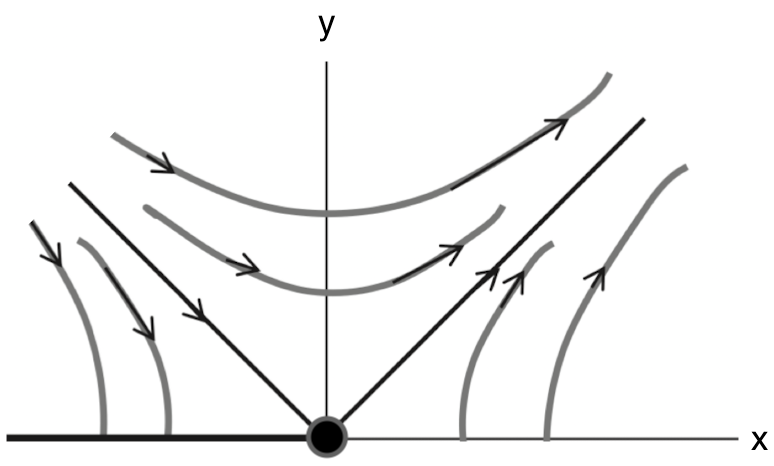
\includegraphics[hsmash=c,width=0.45\linewidth]{pics/LL-RG-flow}
	\caption{KT RG-flow.}
	\label{fig:FL-RG-flow}
\end{figure}

We see that there are three regimes of the RG flow: in the weak interacting regime, the field theory flows to the Tomonaga-Luttinger (TL) line; for strong interaction, depending on the sign of $y$, the systems develop two charge-density-wave (CDW) order, namely the Neel-CDW and Peierls-CDW.


\subsection{Phase Diagram}

\subsubsection{Tomonaga-Luttinger Liquid}
When $K<\frac{1}{2}$, the interacting cosine term become irrelevant.
In this case, the system is in a liquid state, called the \textit{Tomonaga-Luttinger liquid}.
The system on the TL line is described by the non-interacting Hamiltonian:
\begin{equation}
	H = \int \frac{dx}{K} \frac{1}{2}\left[K \Pi^2 + \frac{1}{K}(\partial_x\phi)^2 \right],
\end{equation}
As discussed, we can define a new set of variables to map the Hamiltonian to that of the original bosonic model:
\begin{equation}
\begin{aligned}
	\phi' &= \frac{\phi'_-+\phi'_+}{\sqrt 2} = \frac{\phi}{\sqrt{K}} = \frac{\phi_-+\phi_+}{\sqrt{2K}} \\
	\theta' &= \frac{\phi'_--\phi'_+}{\sqrt 2} = \sqrt{K} \theta = \sqrt{\frac{K}{2}}(\phi_--\phi_+).
\end{aligned}
\end{equation}
The fermion mode is
\begin{equation}
\begin{aligned}
	\psi_{\pm}(x) &= \frac{1}{\sqrt{2\pi a}} \exp\left[-i\sqrt{2\pi} \phi'_{\pm}(x) \right] \\
	&= \frac{1}{\sqrt{2\pi a}} \exp\left\{-i\sqrt{2\pi} \left[K_\pm \phi_+(x)+ K_\mp \phi_-(x) \right]\right\},
\end{aligned}
\end{equation}
where 
\begin{equation}
	K_\pm \equiv \frac{K^{\frac{1}{2}} \pm K^{-\frac{1}{2}}}{2}.
\end{equation}
The Greens function is (assume $\tau>0$):
\begin{equation}
	-G_{\pm}(x,\tau) 
	= \frac{1}{2\pi a} e^{2\pi \langle \phi'_\pm(x,\tau)\phi'_\pm(0) - \phi'_\pm(0)\phi'_\pm(0) \rangle}
\end{equation}
The bosonic correlation is
\begin{equation}
\begin{aligned}
	\langle \phi'_\pm(x,\tau)\phi'_\pm(0) \rangle
	&= K_\pm^2 \langle \phi_+(x,\tau)\phi_+(0)\rangle + K_\mp^2 \langle\phi_-(x,\tau)\phi_-(0)\rangle \\
	&= \frac{K_\pm^2}{2\pi}\ln \frac{L/2\pi}{a-ix+\tau} + \frac{K_\mp^2}{2\pi}\ln \frac{L/2\pi}{a+ix +\tau}
\end{aligned}
\end{equation}
So that
\begin{equation}
\begin{aligned}
	-G_{\pm}(x,\tau) 
	&= \frac{1}{2\pi a} \left[\frac{a}{a + \tau - ix}\right]^{K_\pm^2} \left[\frac{a}{a + \tau + i x}\right]^{K_\mp^2} \\
	&= \frac{1}{2\pi} \frac{1}{a + \tau \mp ix} \left[\frac{a^2}{a^2+x^2+\tau^2}\right]^{K_-^2}
\end{aligned}
\end{equation}
Note that when $K=0$, $K_-=0$, and the theory agrees with the free fermion prediction:
\begin{equation}
	-G(x, 0^+) = \frac{1}{2\pi} \frac{1}{a-ix}
	= \int \frac{dk}{2\pi} e^{ikx-ak} \theta(k)
\end{equation}
However, when $K_- \ne 0$, the additional factor will smear the pole to a brach cut. 
To see this, note that from the dimensional analysis, the Green's function is of anomalous dimension $-K_-^2$.
In the momentum space, this means that the Green's function scales as
\begin{equation}
	G(k,\omega) \sim (k,\omega)^{K_-^2}.
\end{equation}
This implies that the density 
\begin{equation}
	n(k) = n_0 + c k^{K_-^2}.
\end{equation}


\subsubsection{Charge Density Wave Order}
We first consider the case where $y>0$ is sufficiently large. 
Consider
\begin{equation}
	\cos\left[\sqrt{16\pi}\phi(x)\right] = \frac{1}{2} - \sin^2\left[\sqrt{4\pi}\phi(x)\right].
\end{equation}
The energy is minimized if 
\begin{equation}
	\sin\left[\sqrt{4\pi}\phi(x)\right] = \pm 1.
\end{equation}
Note that in our bosonization dictionary,
\begin{equation}
	\psi_{\pm}^\dagger(x)\psi_{\mp}(x) = \frac{1}{2\pi a} e^{\pm i\sqrt{4\pi}\phi(x)},
\end{equation}
so that
\begin{equation}
	\frac{i}{\pi a} \sin\left[\sqrt{4\pi}\phi(x)\right] = \psi_{+}^\dagger(x)\psi_{-}(x)-\psi_{-}^\dagger(x)\psi_{+}(x).
\end{equation}
We know for the Neel-CDW phase, the order parameter is
\begin{equation}
	i\left\langle \psi_{+}^\dagger(x)\psi_{-}(x)-\psi_{-}^\dagger(x)\psi_{+}(x) \right\rangle.
\end{equation}

On the other hand, for $y<0$, consider
\begin{equation}
	\cos\left[\sqrt{16\pi}\phi(x)\right] = -\frac{1}{2} + \cos^2\left[\sqrt{4\pi}\phi(x)\right].
\end{equation}
The energy is minimized if 
\begin{equation}
	\cos\left[\sqrt{4\pi}\phi(x)\right] = \pm 1.
\end{equation}




\subsection{One-dimensional Hubbard Model}
Now we consider the fermion with spin.
The Hubbard model has a non-interacting part,
\begin{equation}
	H_{0}=-\frac{1}{2} \sum_{s, n}\left[\psi_{s}^{\dagger}(n) \psi_{s}(n+1)+\text { h.c. }\right]+\mu \sum_{s, n} \psi_{s}^{\dagger}(n) \psi_{s}(n),
\end{equation}
where $s=\uparrow, \downarrow$ are two possible spin orientations. We do not assume $k_F = \frac{\pi}{2}$ at this point, and use a general chemical potential $\mu$.
Following the usual route, we get two copies of the spinless model:
\begin{equation}
	H_{0}=\sum_{s} \int \frac{d k}{2 \pi} (\mu-\cos k) \psi_{s}^{\dagger}(k) \psi_{s}(k),
\end{equation}
and the continuum version:
\begin{equation}
\begin{aligned}
	H_0 &= v_F \sum_{s} \int d x \left[
		\psi_{s+}^{\dagger}(x)\left(-i \partial_{x}\right) \psi_{s+}(x) +
		\psi_{s-}^{\dagger}(x)\left( i \partial_{x}\right) \psi_{s-}(x)
	\right] \\
	&= \frac{v_F}{2} \sum_s \int d x \left[\Pi_{s}^{2}+\left(\partial_x \phi_{s}\right)^{2}\right].
\end{aligned}
\end{equation}
Let us now turn on the Hubbard interaction,
\begin{equation}
	H_{\mathrm{int}}=U \sum_{n} \psi_{\uparrow}^{\dagger}(n) \psi_{\uparrow}(n) \psi_{\downarrow}^{\dagger}(n) \psi_{\downarrow}(n),
\end{equation}
where $\psi_{\uparrow}, \psi_{\downarrow}$ stand for the original non-relativistic fermion. 
The Hubbard interaction is just the extreme short-range version of the screened Coulomb potential between fermions. 
Due to the Pauli principle, only opposite-spin electrons can occupy the same site.

Let us now express this interaction in terms of the Dirac fields:
\begin{equation}
	\psi_{\uparrow}^{\dagger}  \psi_{\uparrow} \psi_{\downarrow}^{\dagger} \psi_{\downarrow} 
	= \left[\psi_{\uparrow+}^{\dagger} \psi_{\uparrow+}+\psi_{\uparrow-}^{\dagger} \psi_{\uparrow-}+
	\left(\psi_{\uparrow+}^{\dagger} \psi_{\uparrow-} e^{-2 i K_{\mathrm{F}} n}+\text{h.c.}\right)\right] 
	\times(\uparrow \rightarrow \downarrow).
\end{equation}
If we expand out the products and keep only the parts with no rapidly oscillating factors, we will, for generic $k_F$, get the following terms:
\begin{equation}
	H_{\mathrm{int}} = U\left(j_{0 \uparrow} j_{0 \downarrow}\right) + U\sum_n \left(\psi_{\uparrow+}^{\dagger}(n) \psi_{\uparrow-}(n) \psi_{\downarrow-}^{\dagger}(n) \psi_{\downarrow+}(n)+\text{h.c.}\right),
\end{equation}
where
\begin{equation}
	U\left(j_{0 \uparrow} j_{0 \downarrow}\right)
	= \sum_n \left(\psi_{\uparrow+}^{\dagger} \psi_{\uparrow+}+\psi_{\uparrow-}^{\dagger} \psi_{\uparrow-}\right)\left(\psi_{\downarrow+}^{\dagger} \psi_{\downarrow+}+\psi_{\downarrow-}^{\dagger} \psi_{\downarrow-}\right)
\end{equation}
If we now bosonize these terms as per the dictionary, we get, in the continuum,
\begin{equation}
	H_{\mathrm{int}} = U\left[\frac{\partial_x \phi_{\uparrow} \partial_x \phi_{\downarrow}}{\pi}+\frac{1}{2\pi^{2} \alpha^{2}} \cos \sqrt{4 \pi}\left(\phi_{\uparrow}-\phi_{\downarrow}\right)\right]
\end{equation}
We can now separate the theory into two parts by introducing charge and spin fields $\phi_{c}$ and $\phi_{s}$:
\begin{equation}
	\phi_{c/s}=\frac{\phi_{\uparrow} \pm \phi_{\downarrow}}{\sqrt{2}}.
\end{equation}
The parametrization bring the first term in the interaction to a free theory:
\begin{equation}
\begin{aligned}
	\partial_x \phi_{\uparrow} \partial_x \phi_{\downarrow}
	&= \frac{1}{2} \partial_x (\phi_{c}+\phi_s) \partial_x (\phi_c-\phi_s) \\
	&= \frac{1}{2} \left[(\partial_x \phi_c)^2 + (\partial_x \phi_s)^2\right].
\end{aligned}
\end{equation}
The Hamiltonian then become decoupled:
\begin{equation}
	H =H_{c}+H_{s},
\end{equation}
where the charge and spin part of the Hamiltonian are:
\begin{equation}
\begin{aligned}
	H_{c} &=\int \frac{dx}{2 K_c}\left[K_{c} \Pi_{c}^{2}+\frac{1}{K_{c}}\left(\partial \phi_{c}\right)^{2}\right], \\
	H_{s} &=\int \frac{dx}{2 K_s} \left[K_{s} \Pi_{s}^{2}+\frac{1}{K_{s}}\left(\partial \phi_{s}\right)^{2}+\frac{U}{2 \pi^{2} \alpha^{2}} \cos \sqrt{8 \pi} \phi_{s}\right],
\end{aligned}
\end{equation}
where 
\begin{equation}
	K_{c / s} =\frac{1}{\sqrt{1 \pm \frac{U}{\pi}}}.
\end{equation}
The fact that $K_{s} \neq K_{c}$ means that charge and spin move at different velocities. 
This \textit{spin-charge separation} cannot be understood in terms of interacting electrons whose charge and spin would be irrevocably bound. 
This is more evidence of the demise of the quasiparticle, adiabatically connected to the primordial fermion.





\end{document}


